% ---
% Reemplaza líneas 3097–3252 de Docs/Technical_Report.tex.
% Decisiones que lo respaldan: D-005, D-006, H-050.
% Capítulo 4 desde el 2026-10-14 (antes §5).
% ---

\subsection{Análisis de variables clínicas}

\subsubsection{Densidad mamaria}

La distribución de densidad mamaria clasificada por el radiólogo
según patología y tipo de hallazgo se ilustra en la
Figura~\ref{fig:breast_density} del Anexo~\ref{anx:figuras_eda}.

% fuente: D-005; 1_EDA.ipynb
La densidad mamaria más frecuente en el dataset es
la categoría 2 (tejido disperso). El análisis de
correlación confirmó que la densidad mamaria tiene
una correlación casi nula con la etiqueta de
patología ($r = -0.03$ para masas, $r = +0.09$ para
calcificaciones), lo que indica que la densidad
no predice la malignidad de la lesión. Sin embargo,
se observó una correlación negativa moderada entre
densidad y \textit{subtlety} ($r = -0.31$ para masas),
confirmando que las lesiones son más difíciles de
detectar visualmente en tejidos más densos, donde
el tejido glandular camufla las estructuras anómalas.

\subsubsection{Lateralidad y vista mamográfica}

La distribución de lateralidad anatómica y proyección mamográfica
se presenta en la Figura~\ref{fig:laterality_view} del
Anexo~\ref{anx:figuras_eda}.

% fuente: D-005; 1_EDA.ipynb
La distribución de lateralidad es prácticamente
simétrica (1\,819 casos izquierdos vs.\ 1\,749
derechos, ratio 1.04:1), lo que indica ausencia de
sesgo de adquisición por lado. El ligero predominio
de la vista MLO sobre la CC (1\,896 vs.\ 1\,672)
es esperado clínicamente, dado que la vista
MLO captura mayor volumen de tejido mamario
incluyendo la región axilar.

\subsubsection{Morfología de masas}

La Figura~\ref{fig:mass_morphology} muestra la
distribución de forma y margen de las masas por
patología.

\begin{figure}[htbp]
  \centering
  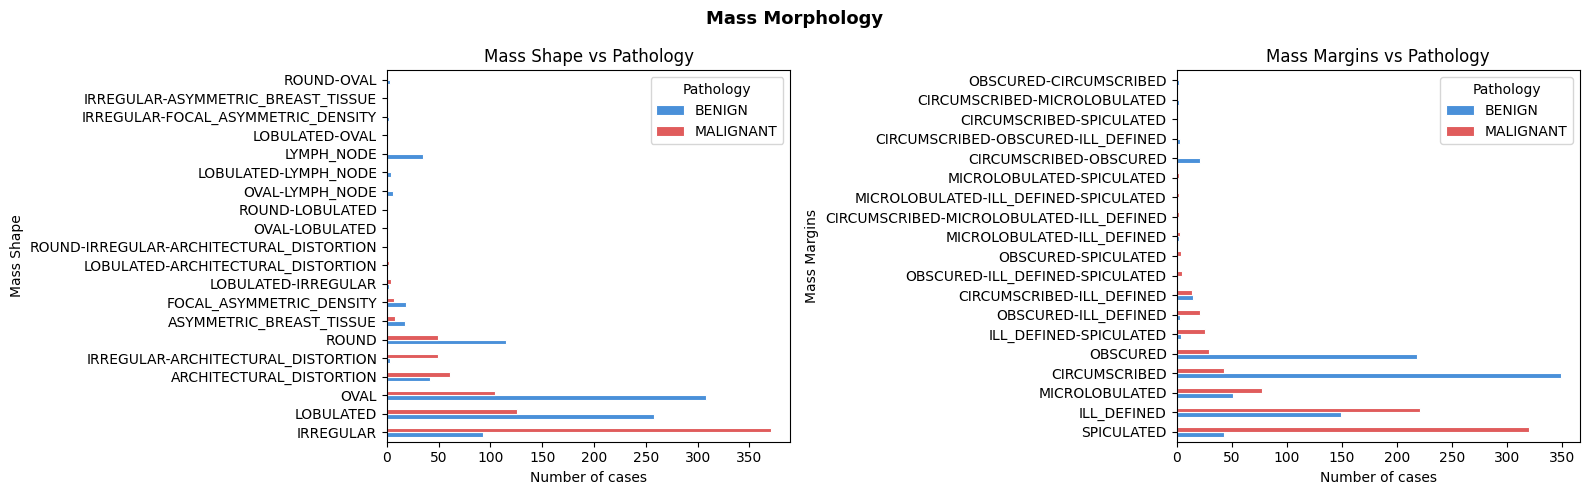
\includegraphics[width=\textwidth]{Figures/C3_mass_morphology.png}
  \caption{Distribución de forma y margen de masas por patología (benigno / maligno).}
  \label{fig:mass_morphology}
\end{figure}

Los resultados revelan una separación morfológica
marcada entre clases. Las masas malignas se asocian
predominantemente con formas \textit{IRREGULAR} y
márgenes \textit{SPICULATED}, patrón clínico clásico
del carcinoma invasivo, donde el tumor crece
desordenadamente con extensiones hacia el tejido
circundante. Las masas benignas presentan formas
\textit{OVAL} con bordes \textit{CIRCUMSCRIBED},
patrón típico de fibroadenomas o quistes encapsulados.
Esta separación morfológica sugiere que las
características extraídas de masas deberían ser
intrínsecamente más separables en cualquier espacio
de representación, incluyendo el espacio de Hilbert
cuántico generado por los \textit{feature maps}.

\subsubsection{Morfología de calcificaciones}

La Figura~\ref{fig:calc_morphology} presenta la
distribución de tipo y distribución de las
calcificaciones por patología.

\begin{figure}[htbp]
  \centering
  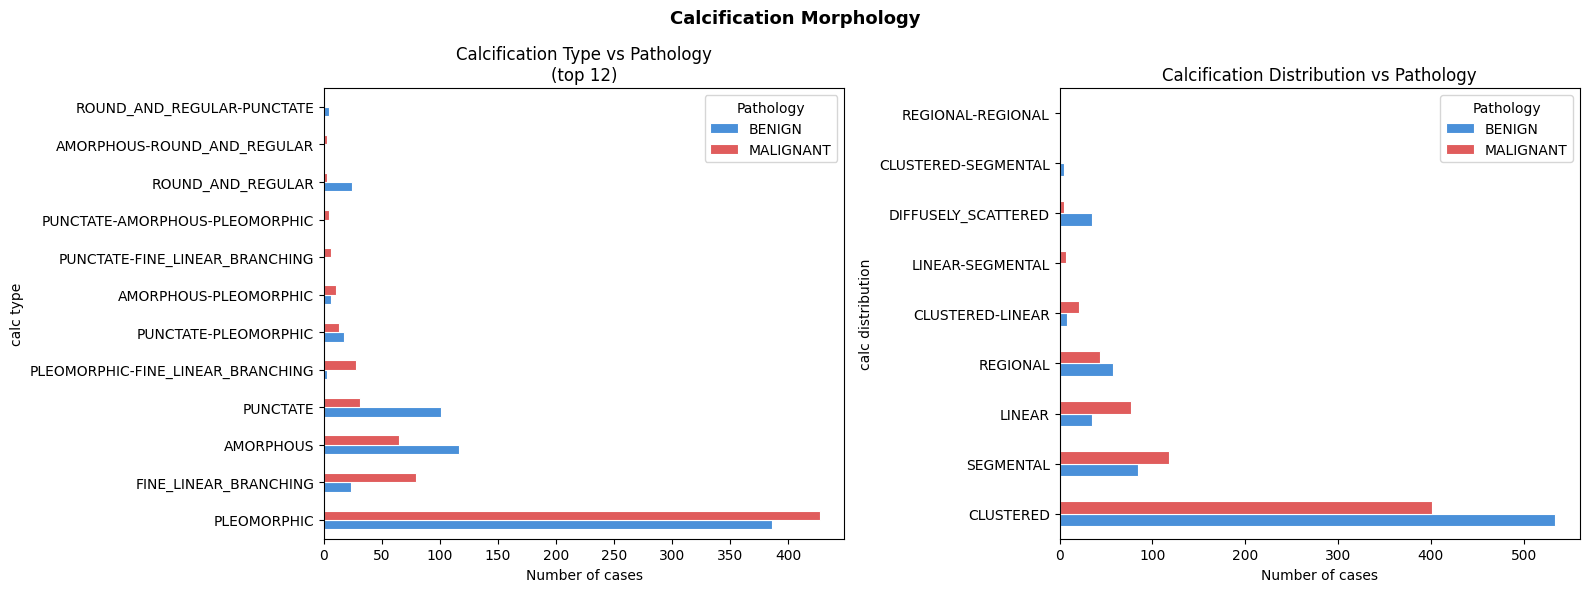
\includegraphics[width=\textwidth]{Figures/C4_calc_morphology.png}
  \caption{Distribución de tipo y distribución espacial de calcificaciones por patología.}
  \label{fig:calc_morphology}
\end{figure}

A diferencia de las masas, las calcificaciones
presentan el tipo morfológico más frecuente
(\textit{PLEOMORPHIC}) compartido entre ambas clases.
Este solapamiento morfológico implica que las
calcificaciones constituyen un problema de
clasificación más exigente que las masas en cuanto a
los descriptores categóricos del radiólogo. Este
escenario es relevante para el presente trabajo
porque permite contrastar el efecto de las
transformaciones cuánticas en dos subproblemas de
dificultad distinta.
% Corregido el 2026-10-19 (auditoría A5-2): el texto de TT1 anticipaba que la codificación cuántica
% «puede revelar estructura discriminativa no accesible para los métodos clásicos», en contradicción
% con §2.1.6 y §6; además, con las 67 características radiómicas las calcificaciones resultan más
% separables que las masas (§6.5), así que la menor separabilidad vale solo para los descriptores.

\subsubsection{Correlaciones entre variables clínicas}

La Figura~\ref{fig:correlation_matrix} presenta la
matriz de correlación de las variables clínicas
numéricas del dataset.

\begin{figure}[htbp]
  \centering
  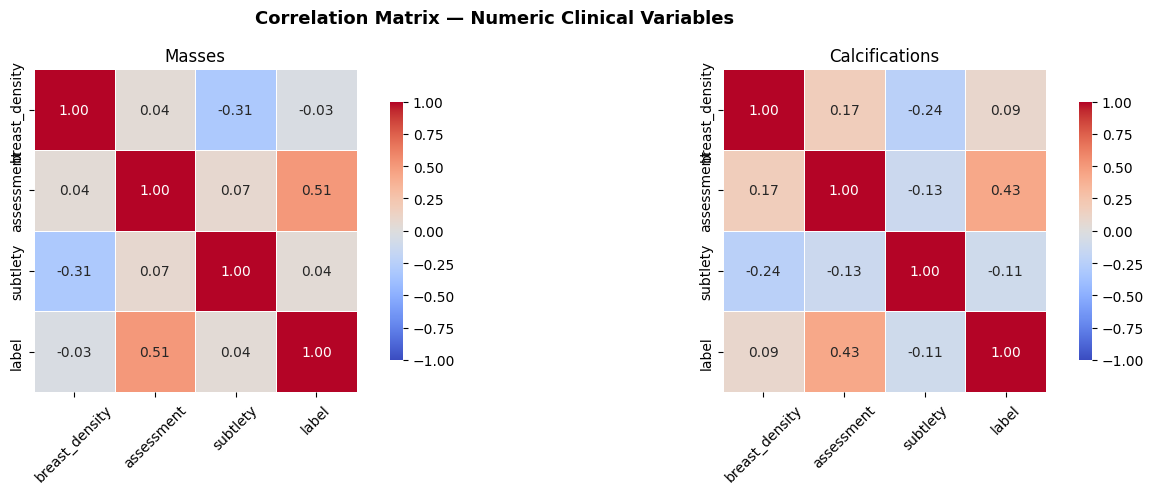
\includegraphics[width=\textwidth]{Figures/C5_correlation_matrix.png}
  \caption{Matriz de correlación de variables clínicas numéricas por tipo de hallazgo.}
  \label{fig:correlation_matrix}
\end{figure}

% fuente: D-005; 1_EDA.ipynb
La variable \texttt{assessment} (categoría BI-RADS)
presenta la correlación más alta con la etiqueta de
patología ($r = +0.51$ para masas, $r = +0.43$ para
calcificaciones), lo cual es esperado dado que el
BI-RADS fue diseñado precisamente como escala de
sospecha de malignidad. Sin embargo, esta variable
no puede utilizarse como \textit{feature} de entrada
al modelo porque constituye \textit{data leakage}:
es una etiqueta clínica derivada de la imagen, no
una característica morfológica independiente.

% fuente: D-005, D-006; 1_EDA.ipynb
Las variables \texttt{breast\_density} y
\texttt{subtlety} presentan correlaciones
prácticamente nulas con la etiqueta de patología
($|r| < 0.12$ en todos los casos), confirmando que
el poder predictivo reside en las características
morfológicas de la imagen y no en los metadatos
clínicos del CSV. Este resultado valida la decisión
metodológica de extraer \textit{features} directamente
de las imágenes DICOM mediante PyRadiomics.
